Uma combinação simples é um subconjunto com k elementos de um conjunto universo com n elementos. É interessante ressaltar a ideia de conjunto pois a ordem dos elementos de um subconjunto não altera sua identidade, ou seja, um subconjunto $\{a, b, c\}$ é o mesmo que $\{c , a, b\}$.

Representado pelo símbolo matemático $\mathrm{C}_k^n$, que significa ``o número de combinações, tomadas $k$ a $k$, que podem se selecionadas de um total de $n$ objetos distintos''.  É esperado que $k \leq n$, visto que estamos calculando o número de maneiras de escolher $k$ objetos de um total $n$.

Sabemos que uma coleção de n objetos pode ser ordenada de $n!$ jeitos. Caso quiséssemos organizar esses $n$ objetos no intervalo de $k$ a $n$ teríamos um arranjo com repetição dado pela fórmula $ \dfrac{n!}{(n - k)!}$ estudada anteriormente. Então se quiséssemos calcular as maneiras de selecionar esses objetos de forma que a ordem deles não importasse, ou seja, uma ordem $\{a, b, c\}$ sendo o mesmo que $\{c , a, b\}$, teríamos então que remover a quantidade de permutações entre esses objetos, dividindo pelo número de formas que eles se arranjam entre si, dessa forma teríamos $\dfrac{\dfrac{n!}{n-k}}{k!}$o que nos induz a fórmula $\dfrac{n!}{k!(n-k)}$.

\subsection*{Questão 1}

\begin{wrapfigure}{l}{0.4\textwidth}
	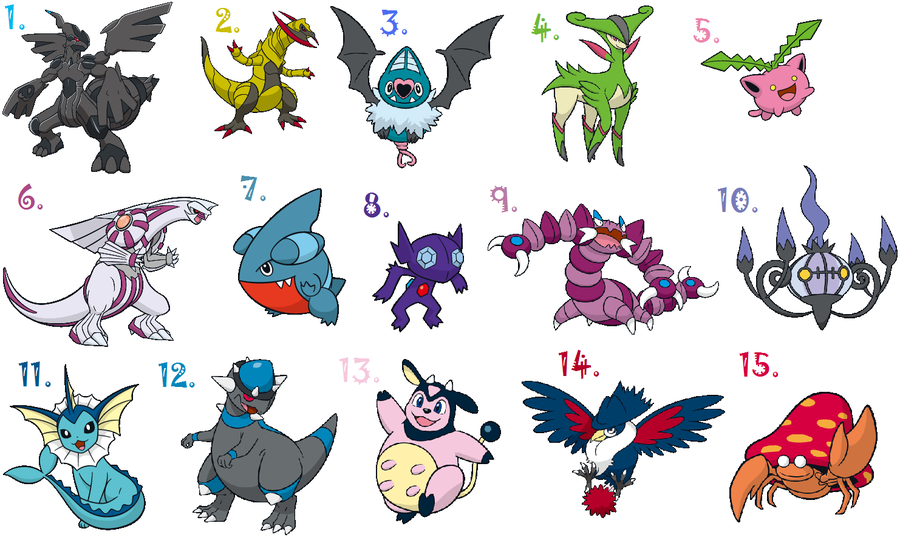
\includegraphics[width=5cm, left]{imagens/pokemon.png}
\end{wrapfigure}

Um treinador pokemon possui a sua disposição 15 pokemons, mas ele só pode carregar 6 pokemons de cada vez, então ele decidiu contar de quantas maneiras diferentes ele poderia escolher um time com 6 dessas criaturinhas.

\subsubsection*{Resolução da questão 1}

Note que o treinador não se atentou aos tipos de pokemons que dispunha, dessa forma ele só quer calcular o número de combinações que formam um time de 6, o que pode ser facilmente calculado pela fórmula mostrada anteriormente: $\dfrac{15!}{6!(15-6)}$, o que resulta em um total de 5005 maneiras de formar times pokemons.

\subsection*{Questão 2}

\begin{wrapfigure}{l}{0.4\textwidth}
	
\includegraphics[width=5cm, left]{imagens/mst.png}
\end{wrapfigure}

(UFSM) A reforma agrária ainda é um ponto crucial para se estabelecer uma melhor distribuição de renda no Brasil. Uma comunidade de sem-terra, após se alojar numa fazenda comprovadamente improdutiva, recebe informação de que o INCRA irá receber uma comissão para negociações. Em assembléia democrática, os sem-terra decidem que tal comissão será composta por um presidente geral, um porta-voz que repassará as notícias à comunidade e aos representantes e um agente que cuidará da parte burocrática das negociações. Além desses com cargos específicos, participarão dessa comissão mais 6 conselheiros que auxiliarão indistintamente em todas as faces da negociação.
Se, dentre toda a comunidade, apenas 15 pessoas forem consideradas aptas aos cargos, o número de comissões distintas que poderão ser formadas com essas 15 pessoas é obtido pelo produto

\subsubsection*{Resolução da questão 2}

Existem os 3 cargos principais para serem preenchidos pelos 15 sem-terra, assim como os 6 cargos restantes de conselheiros, sendo assim, iremos ter 15 pessoas concorrendo aos cargos principais e depois de preencher esses cargos, 12 pessoas estarão concorrendo a conselheiros.

Note que, para a posição dos cargos principais é importante, ou seja, as pessoas a, b e c, por ocuparem cargos diferentes formam novos grupos, então temos que distribuir os 15 sem-terra entre os 3 cargos, tendo então 15 possibilidades de escolha para presidente, 14 para porta-voz e 13 para agente, totalizando $15 \cdot 14 \cdot 13$ arranjos desses cargos.

Para os cargos de conselheiros um grupo contendo as pessoas ``a, b, c, d'' e ``e'' são o mesmo grupo, não importa a ordem de disposição dos sem-terra, dessa forma teríamos uma combinação das 12 pessoas restantes para um grupo de 6, utilizando a fórmula teremos $\dfrac{12!}{6!(12-6)}$ que implica em $11 \cdot 7 \cdot 3 \cdot 2^{2}$.

Contabilizando as possibilidades de conselheiros e cargos principais teremos  $15 \cdot 14 \cdot 13 \cdot 11 \cdot 7 \cdot 3 \cdot 2^{2}$ formas de organizar comissões distintas formadas pelos 15 sem-terra.
